\documentclass[assd_tp2_main.tex]{subfiles}

\begin{document}

\section{Síntesis de sonidos mediante modelos f\'isicos}
Se analizarán dos variantes del modelo Karplus-Strong en paralelo, tanto de manera teórica como práctica. 

\subsection{Análisis de transferencias}

\subsubsection{Bloque A Elemental}
Se resolverá, como cálculo auxiliar un bloque sencillo definido como:
\begin{figure}[H]	
	\centering
	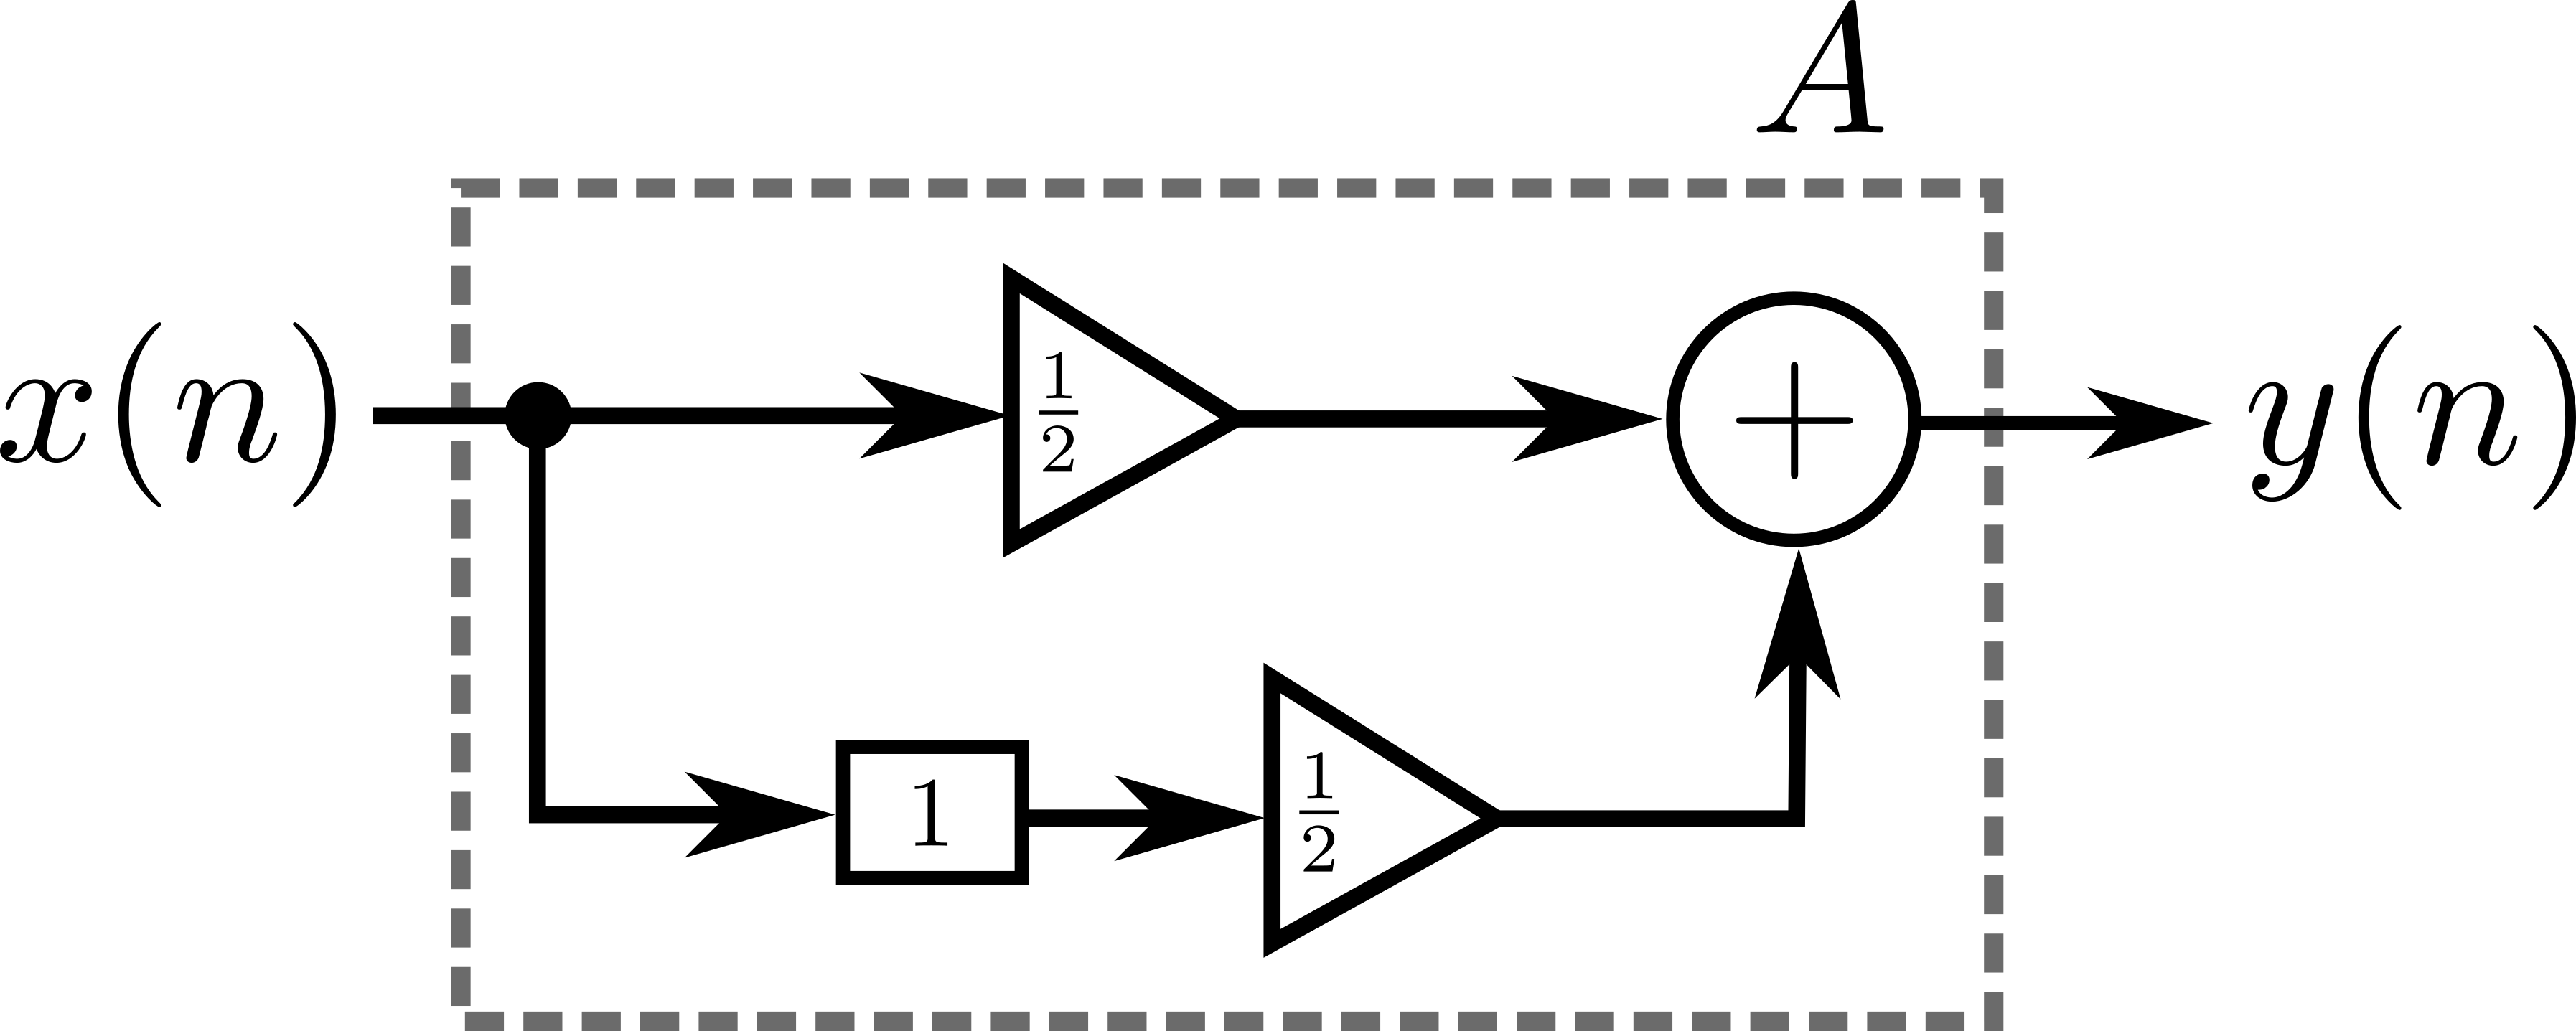
\includegraphics[scale=1]{graficos/bloque1ej5.png}
	\caption{Bloque elemental}
	\label{fig:bloqueElemental}
\end{figure}

Este bloque solo promedia los dos ultimos valores de entrada. Su transferencia esta dada por
\begin{equation}
x(n)=\frac{1}{2}x(n)+\frac{1}{2}x(n-1)
\end{equation}
\begin{equation}
Y(z)=\frac{1}{2}X(z)+\frac{1}{2}X(z)z^{-1} \implies A(z)=\frac{Z+1}{Z}
\end{equation}
Se puede observar que el bloque A es pasa-bajos (cero en $Z=-1$); lo cual es, en principio, razonable, el bloque A suaviza la entrada.

\subsubsection{Karplus Strong 1}
Se resolverá un nuevo sistema, el cuál consiste en una adicion de realimentación al sistema anterior
\begin{figure}[H]	
	\centering
	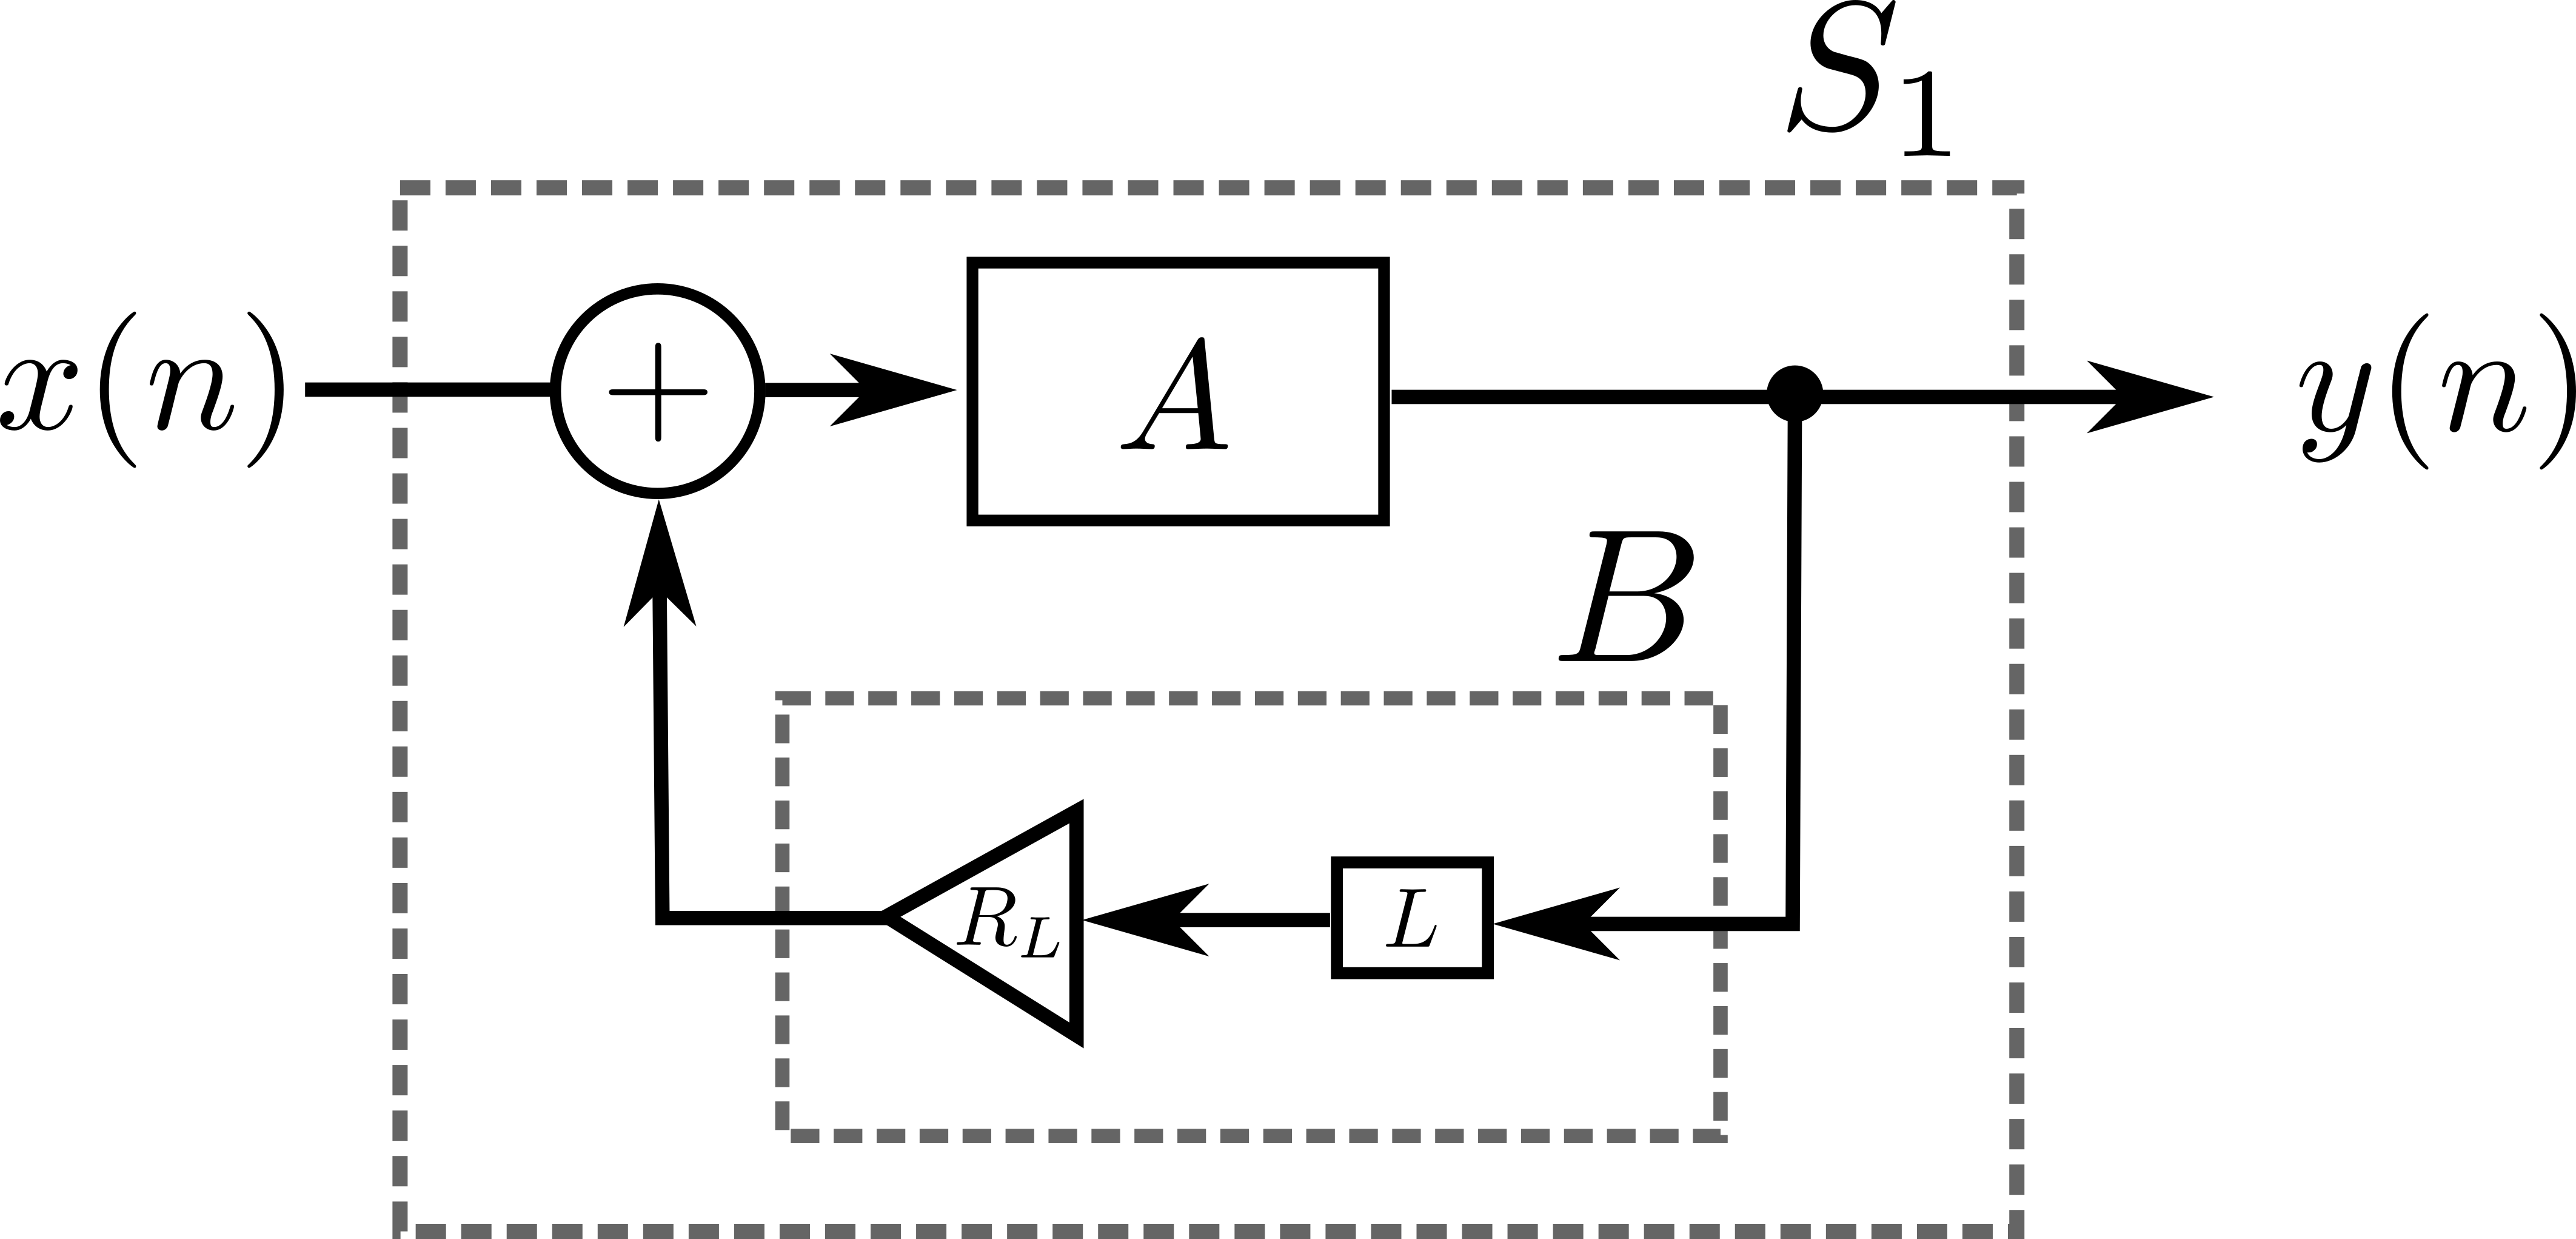
\includegraphics[scale=1]{graficos/bloque2ej5.png}
	\caption{Bloque elemental}
	\label{fig:bloqueElemental}
\end{figure}

Mediante teória de feedback, considerando que $B(z)=Z^{-L}R_L$ se llega a que
\begin{equation}
S_1(z)=\frac{}{}
\end{equation}

\end{document}

